\section{Directed Khepera (class)}

\subsection{Introduction}

This class aims to pilot the Khepera to a given (x,y) position. To do 
so, we get the position and orientation of the Khepera from a camera 
hanging from the ceiling. It needs to calculate the needed orientation 
to drive to a (x,y) position and sends a command to the Khepera via a 
serialport to make it turn or drives forward.

\subsection{Communication}

It first opens a port for serial port communication. The serialport 
communicates via Bluetooth. In Ubuntu, it is usually “/dev/rfcomm0”.

To write commands to the buffer, it is imperative to add a carriage ‘\r’ 
at the end. If not, the Khepera will not recognize the command. 

The buffer is read char by char. The robot always answers to commands. 
The buffer is emptied after every command that is sent.

\subsection{Navigation}

    \marginpar{
        \captionof{figure}{Navigation based on desired angle}
        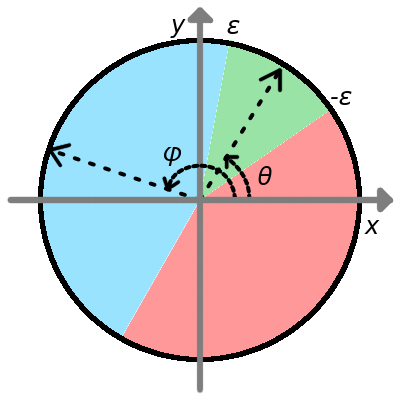
\includegraphics[width=5cm]{./img/desiredangle.png}
        The orientation $\theta$ is the angle between the
        line $\overline{CD}$ and the $x$ axis. It ranges
        counterclockwise from 0 to 2$\pi$.
    }
 
    \begin{enumerate}
        \item It first get the position of the robot including 
            the orientation. 
        \item If the detection is not successful and position is unknown, 
            it sends a command to immobilize the robot
        \item It then calculates the desired angle with desired\_angle = 
            atan2(y-new\_y,x-new\_x)
        \item It add PI to the calculated angle and the robot orientation 
            to get range (0,2PI) rather than (–PI,PI)
        \item Angle error = desired\_angle – robot\_angle
        \item If the angle error is absolutely smaller than epsylon 
            ( abs(angle\_error) < epsilon) it sends a forward command
        \item If the absolute angle\_error is between epsilon and PI is 
            sends a turn right command
        \item Else send a turn left command
        \item Do this while $(x-new\_x)^2+(y-new\_y)^2 > epsilon^2$ 
    \end{enumerate}


The turn right and turn left commands are graded on the level of angle 
error. To simplify calculations, negative angles are inverted by adding 
2*PI before calculating turning speed. The function of the speed is 
the following:

Speed = angle*(\_max\_speed-\_min\_speed)/(PI-angle\_threshold) + 
(PI*\_min\_speed-angle\_threshold*\_max\_speed)/(PI-angle\_threshold)

\subsection{Improvements}

There is no command for the robot for a definite angle rotation. It 
would be a great enhancement for the rapidity and accuracy of the robot 
movements if we could find a way to make it precise turns of a given 
angle with a single command. There is a command to make a precise turn 
of the wheels, but it doesn’t interpolate directly to a complete robot 
rotation of a precise angle. We would need to calculate how much the 
Khepera moves for a precise rotation of the wheels.

The update of the tapir detector and the time between read/write commands 
on the buffer of the serial port are really slow. The tapir detector 
seems to update values at a rate between 1 to 2 times per second, 
which is incredibly slow. It would be really helpful to speed up both 
processes to get higher accuracy in the navigation.

\subsection{How to use}
The tapir detector must be on. Set parameters of the tapir detector in 
khepera\_tapir.cfg. To learn how to set up the Bluetooth connection, 
take a look at the section khepera the chapter How to make an experiment.

\subsubsection{Constructor parameters}
    \begin{description} \itemindent=-15pt
        \item[PORT] port of the serialport. Usually “/dev/rfcomm0” in 
            Ubuntu.
        \item[Max\_speed, min\_speed (optional)] Be carefull if you set 
            those parameters. The update time of the detector is slow 
            and serial port communication too, so if the max\_speed is 
            too high, there might be overruns.
    \end{description}

\subsubsection{Init parameters}
    \begin{description} \itemindent=-15pt
        \item[manipulate] If true, the robot enters an infinite loop where 
            you can send commands. Write “quit” to end, it then returns 
            false and CLsquare ends.
        \item[delta\_t] The sleep time between each loop of the 
            navigation algorithm. Delta\_t seems to need to be equal 
            or higher than 1.0 second because of the time that 
            take Tapir.update() and write/read serialport commands.
    \end{description}

